\section{Einarbeitung}
\label{sec:Einarbeitung}

Der erste Arbeitstag war organisatorischer Natur. Ich wurde meinem Team vorgestellt und danach noch einmal durch das Gebäude geführt, wo ich die anderen Teams kennenlernte. Ich bekam Einblick in die Poststelle und die mit Tresoren gesicherten Hardware-Lager, welche in der Anfangszeit meinen Arbeitsplatz darstellten. Danach wurde mir der Aufbau des Büros erklärt und mein Arbeitsplatz zugewiesen.
\begin{figure}[H] 
  \centering
     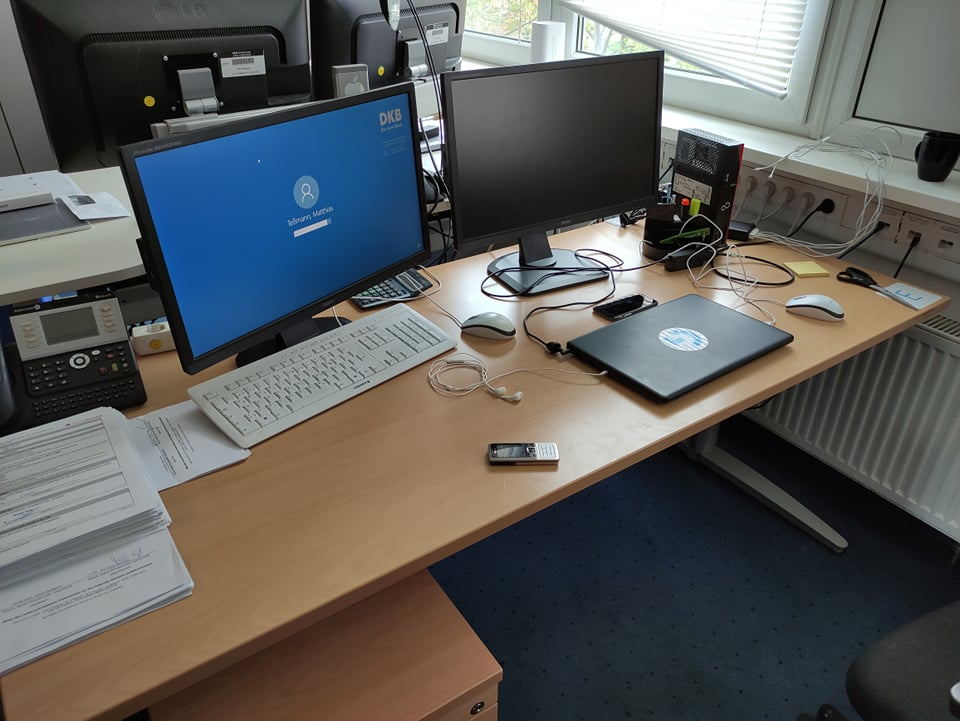
\includegraphics[width=1\textwidth]{arbeitsplatz.jpg}
  \caption{Arbeitsplatz}
  \label{fig:Bild1}
\end{figure}
\noindent
 Der Arbeitsplatz umfasste einen höhenverstellbaren Tisch, zwei Monitore und einen kleinen Stand-Pc (Thin-Client), welcher nur wenig Leistung benötigte, da sich in der DKB-Service über diese Rechner auf einer Citrix-Session eingeloggt und damit komplett arbeitsplatz-unabhängig gearbeitet werden kann. Ich bekam eine Einführung in die Hardware und den Anmeldeprozess. Danach wurden mir per E-Mail die Passwörter zu verschiedenen Programmen und Plattformen mitgeteilt. Zum Abschluss des ersten Tages bekam ich meinen Transponder, welcher sowohl als Zutrittskarte für die mechanisch gesicherten Türen im Gebäude, als auch zum Festhalten der Arbeitszeiten am Check-In dient. Die DKB-Service ermöglicht ihren Mitarbeitern übergreifend Gleitzeit als Stunden-Modell. In den darauffolgenden Arbeitstagen beschäftigte ich mich hauptsächlich mit Schulungen im Bereich IT-Sicherheit, Datensicherheit, \textit{Fraud Prevention and Detection} und Umgang mit dem Kunden. Diese Schulungen sind für jeden Mitarbeiter Pflicht und müssen alle zwei Jahre wiederholt werden. Zum Abschluss der ersten Woche bekam ich meine Hardware, welche aus einem Laptop, einem iPad 10 pro und einem iPhone 8 bestand, um auch von Zuhause arbeiten zu können. Zwischendurch bekam ich meine ersten einfachen Augaben, wobei ich besonders mit dem Updaten der iPads vertraut gemacht wurde. Diese mussten vor dem Ausliefern an die Mitarbeiter immer aktuell sein. Da die Mitarbeiter der DKB hauptsächlich mit Apple-Produkten versorgt wurden und ich bis dato kein iPhone oder Ähnliches besaß, machte ich mich ausführlich mit dem Aufbau von iOS vertraut. Die Woche verging schnell und es gelang mirl einen guten Draht zu den Kollegen aufzubauen, sodass ich mich schon auf die zweite Arbeitswoche freute.

\subsection{IT-Lager}
\label{sec:IT-Lager}

Die zweite Woche begann mit der Einführung in meinen Abreitsbereich für die ersten Wochen. Ich wurde im so genannten IT-Lager eingesetzt, wo die Laptops für Mitarbeiter der Bank mit einem hauseigenen Betriebssystem bespielt wurden.
\begin{figure}[H] 
  \centering
     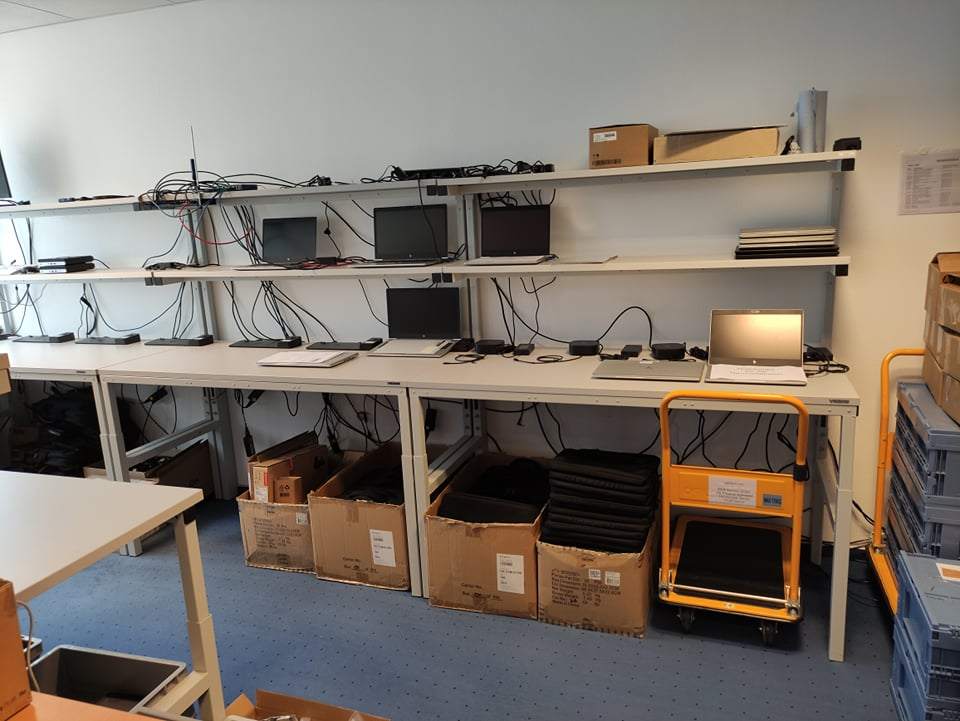
\includegraphics[width=1\textwidth]{itlager.jpg}
  \caption{IT-Lager}
  \label{fig:Bild1}
\end{figure} 
\begin{figure}[H] 
  \centering
     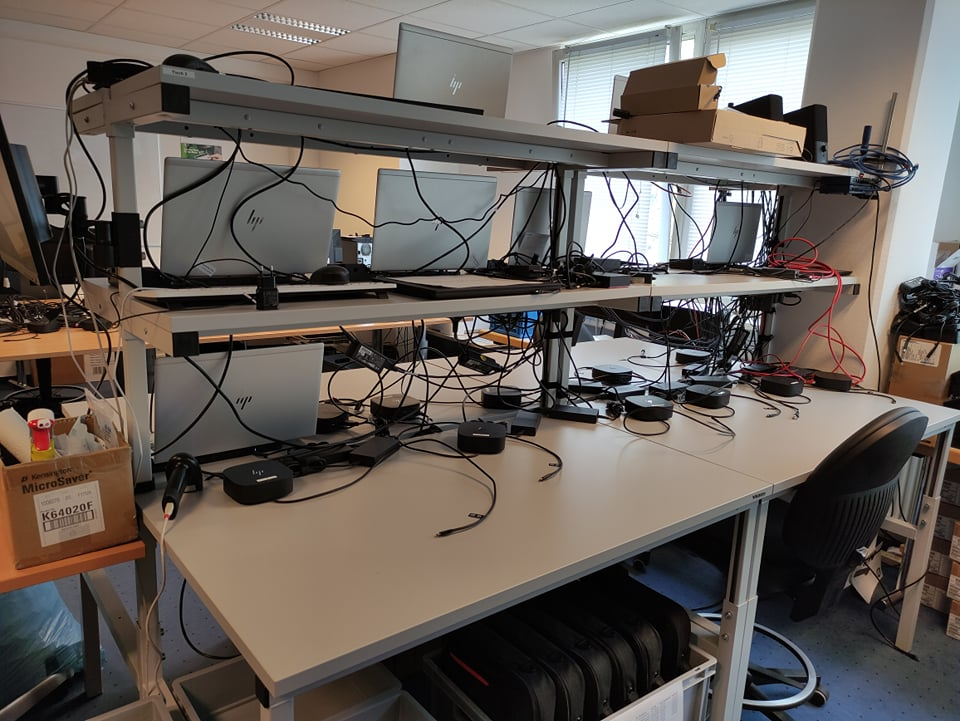
\includegraphics[width=1\textwidth]{itlager1.jpg}
  \caption{IT-Lager}
  \label{fig:Bild1}
\end{figure} 
\noindent
Des Weiteren wurden hier die Laptops gehärtet und die Festplatten verschlüsselt, sodass diese nicht missbraucht werden konnten. Ich wurde in den Ablauf des Aufsetzen eines solchen Rechners eingearbeitet, welcher im Groben daraus bestand, einen neuen Laptop an das Netzwerk anzuschließen und über einen Befehl im Bios-Terminal das Laden des Betriebssystems aus dem Netzwerk zu starten. Danach wurde auf jedem Laptop ein provisorischer Benutzer erstellt, damit die Festplatten verschlüsselt werden konnten. Es musste darauf geachtet werden, dass die Laptops keine Fehlermeldungen warfen, was durchaus vorkommen konnte. Weiterhin wurde mir beigebracht die Laptops entsprechend von Sonderanforderungen aufzurüsten, fachmännisch zu Öffnen und wieder zu Schließen. Ein solches Upgrade umfasste meist das Hinzufügen eines neuen Arbeitsspeicher-Riegels und die Erweiterung um eine neue SSD-Festplatte. Dabei war darauf zu achten sich zu erden bevor man empfindliche Hardware anfasst. Abgeschlossen wurde eine Installation des Laptops mit dem Aufspielen von Norton Security, welches den Laptop mit einem firmeneigenen Profil härtete und die Festplatten verschlüsselte. Ein weiterer Teil der Arbeit dort bestand darin die Hardware entsprechend sorgfältig zu verpacken und an die entsprechenden Mitarbeiter per Hauspost zu verschicken. Verschickt wurde die Hardware aus der Poststelle, welche gleichzeitig ein zweites kleines IT-Lager darstellte.
\begin{figure}[H] 
  \centering
     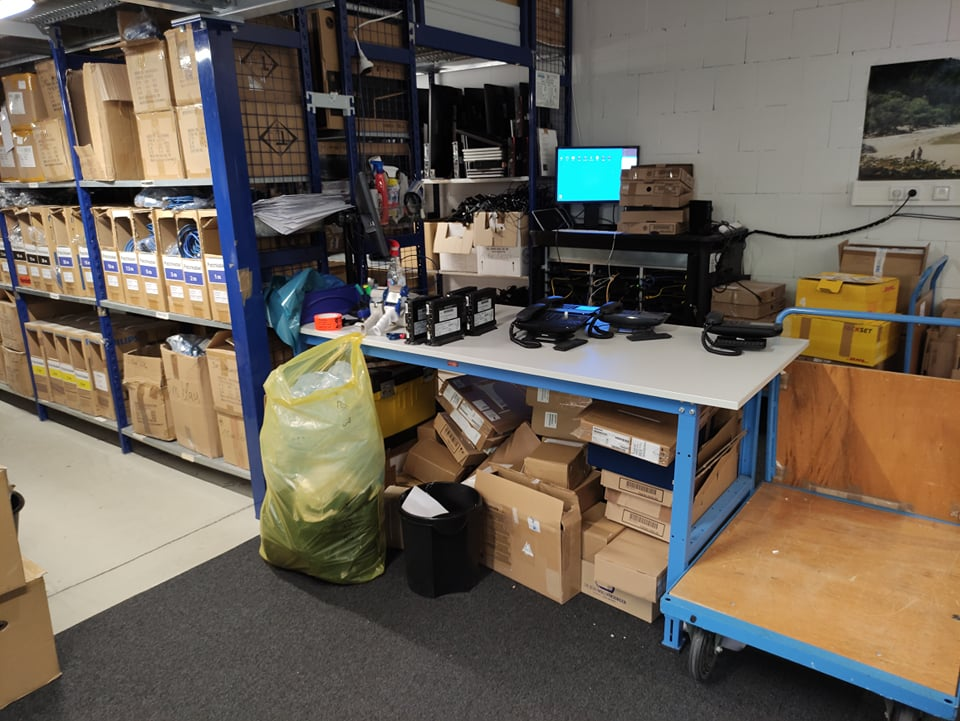
\includegraphics[width=0.9\textwidth]{poststelle.jpg}
  \caption{Poststelle}
  \label{fig:Bild1}
\end{figure} 
\begin{figure}[H] 
  \centering
     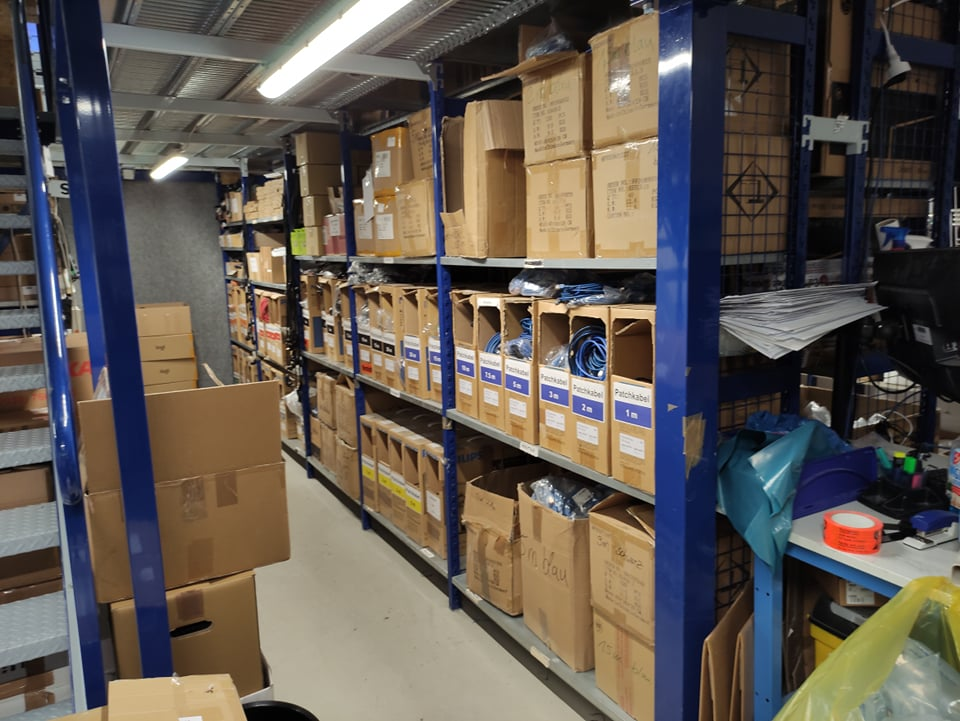
\includegraphics[width=0.9\textwidth]{poststelle1.jpg}
  \caption{Poststelle}
  \label{fig:Bild1}
\end{figure} 
\noindent

 Dort wurde kleinere zusäzliche Hardware wie LAN-Label, Router, Switches, Netzteile, Mäuse, Tastaturen und Steckdosen gelagert. In der Poststelle wurden die Etiketten zum Versand der Hardware ausgedruckt, indem im System der Mitarbeiter gesucht und dann die entsprechende Hardware verbucht wurde. Dazu wurde ein Übergabeprotokoll erstellt, welches die zu übergebenen Hardwarebestandteile auflistete. Dieses diente der Absicherung, dass auch die korrekte Hardware verschickt wurde. Der Mitarbeiter musste das Protokoll unterschreiben, einscannen und an unser Team zurückschicken. Daraufhin wurde ihm der jeweilige PIN oder Entsperrcode übermittelt, damit die Hardware verwendet werden konnte. Im spätere Verlauf versuchte ich den Prozess des Erstellens eines Übergabeprotokolls zu optimieren. Die Arbeit im IT-Lager und in der Poststelle setze das Wissen voraus welche Hardware benötigt wird und welche Ersatzteile zu den jeweiligen Geräten gehören. Dieser Teil befasste sich demnach besonders mit Hardware und den jeweiligen Komponenten. In der Poststelle gab es auch einen Bereich in dem kleinere Reperaturarbeiten an der Hardware durchgeführt werden konnten. Besonders oft benutzt ich dort den Lötkolben, mit dem ich kleinere Reperaturen an Kabeln oder gelösten Lötstellen durchführte. Dabei war besonders wichtig, dass man die richtige Spitze zu der jeweiligen Arbeit auswählte. Auch war darauf zu achten, dass das die Zusammensetzung des Lots für die entsprechende Temepratur geeignet ist und dass die Lötspitze immer sauber gehalten wird.
\\
 Ein Vorgehen beim Verlöten von Bauteilen kann folgendermaßen beschrieben werden:
\\
\begin{itemize}
	\item Die zu verbindenden Drähte verdrillen und Elektrobauelemente rutschfest auf der Platine platzieren.
	\item Ist eine solche Platzierung nicht möglich, das Bauteil mit einer Spitzzange während des Lötens fixieren.
	\item Vor dem eigentlichen Löten die Bauteile durch Berühren mit der Lötspitze auf die richtige Arbeitstemperatur bringen.
	\item Danach das Lot an die Bauteile und mit der heißen Lötspitze zum Schmelzen bringen. Das Lot sollte zwischen die Bauteile fließen, es erkaltet dann silbrig glänzend.
	\item Kommt es während des Lötens zu Erschütterungen der Lötstelle, ist die Verbindung unter Umständen nicht leitfähig. Es handelt sich um eine kalte Lötstelle, die durch Wiederholen des Lötvorgangs nachbearbeitet werden muss. Gründe für eine kalte Lötstelle können auch ein zu schwacher Lötkolben oder zu kalte Kontaktstellen der Bauteile sein. Kalte Lötstellen haben 			eine matte graue Färbung sowie eine raue Oberfläche.
	\item Reste von Lot an der Lötspitze unverzüglich entfernen.
\end{itemize}
\
\\
Zusammenfassend ist zu sagen, dass die Einarbeitungszeit besonders den hardwaretechnischen Bereich abdeckte. So lernte ich den korrekten Umgang mit sensibler Hardware, das Aufrüsten von verschiedesten Computerkomponenten, das Reparieren von einfachen Bauteilen, die Logistik hinter der Ausgabe von Hadrware und den Prozess des Aufsetzens und Härtens eines Rechners für Mitarbeiter kennen. Dieser Teil machte mir persönlich viel Spaß, da er sowohl körperliche Arbeit, als auch Präzision und Fachwissen voraussetze. Besonders die Reperaturarbeiten vermittelten mir ein solides Grundwissen, von dem ich seit dem auch privat profitieren konnte. In dieser Zeit kamen mir besonders der Einführungskurs in Computer Engineering (Löten eines USB-Sticks) und das Projekt Computer Engineering zu Gute, da dort ich dort schon einen ersten Kontakt mit Löten und den Umgang mit Bauteilen hatte. Dieses Grundwissen konnte hier erweitert und vertieft werden und es zeigt sich, dass ich mir vorstellen konnte auch beruflich in diese Richtung zu gehen, da sich diese Arbeit mehr wie ein Hobby als Arbeit anfühlte. 